\documentclass[a4paper,12pt]{article} % тип документа

%  Русский язык
\usepackage[T2A]{fontenc}			% кодировка
\usepackage[utf8]{inputenc}			% кодировка исходного текста
\usepackage[english,russian]{babel}	% локализация и переносы

\usepackage{graphicx}               % импорт изображений
\usepackage{wrapfig}                % обтекаемые изображения
\graphicspath{{pictures/}}          % обращение к подкаталогу с изображениями
\usepackage[14pt]{extsizes}         % для того чтобы задать нестандартный 14-ый размер шрифта
\usepackage[warn]{mathtext}         % русский язык в формулах
\usepackage{indentfirst}            % indent first
\usepackage[margin = 25mm]{geometry}% отступы полей
\usepackage[table,xcdraw]{xcolor}   % таблицы
\usepackage{amsmath,amsfonts,amssymb,amsthm,mathtools} % Математика
\usepackage{wasysym}                % ???
\usepackage{upgreek}                % ???  
\usepackage{caption}
\captionsetup{labelsep=period}
\usepackage{gensymb} % degree symbol
\usepackage{multirow}

\begin{document}
	\begin{center}
		
		\textbf{НАЦИОНАЛЬНЫЙ ИССЛЕДОВАТЕЛЬСКИЙ УНИВЕРСИТЕТ \\ <<МОСКОВСКИЙ ФИЗИКО-ТЕХНИЧЕСКИЙ ИНСТИТУТ>>}
		\vspace{13ex}
		
		\textbf{Лабораторная работа 3.1.3 \\ <<Измерение магнитного поля Земли>> }
		\vspace{60ex}
		
		\normalsize{Овсянников Михаил Александрович \\ студент группы Б01-001\\ 2 курс ФРКТ\\}
	\end{center}
	
	\vfill 
	
	\begin{center}
		г. Долгопрудный\\ 
		2021 г.
	\end{center}
	
	\thispagestyle{empty} % выключаем отображение номера для этой страницы
	
	\newpage
	\setcounter{page}{20}
	
\textbf{Цель работы:} определить характеристики шарообразных неодимовых магнитов и, используя законы взаимодействия магнитных моментов с полем, измерить горизонтальную и вертикальную составляющие индукции магнитного поля Земли и магнитное наклонение.

\textbf{В работе используются:} 12 одинаковых неодимовых магнитных шариков, тонкая нить для изготовления крутильного маятника, медная проволока диаметром (0,5 – 0,6) мм, электронные весы, секундомер, измеритель магнитной индукции АТЕ-8702, штангенциркуль, брусок из немагнитного материала (25$\times$30$\times$60 мм$^3$), деревянная линейка, штатив из немагнитного материала; дополнительные неодимовые магнитные шарики ($\thicksim$ 20 шт.) и неодимовые магниты в форме параллелепипедов (2 шт.), набор гирь и разновесов.

\vspace{7mm}
{\large \textbf{Экспериментальная установка.}}

\textbf{Измерение горизонтальной составляющей индукции магнитного поля Земли}


\begin{figure}[h!]
	\centering
	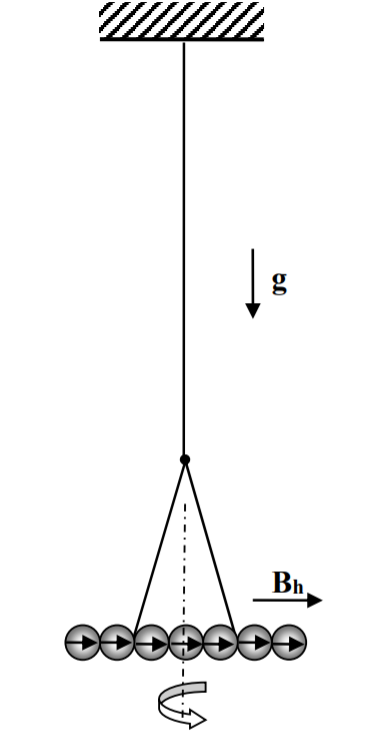
\includegraphics[scale=0.7]{Pictures/Гор.png}
\end{figure}

Магнитное поле Земли в настоящей работе определяется по периоду крутильных колебаний магнитной стрелки вокруг вертикальной оси.

Магнитная стрелка» образована из сцепленных друг с другом противоположными полюсами шариков и с помощью $\Lambda$-образного подвеса подвешена в горизонтальном положении. Под действием вращательного момента магнитный момент «стрелки» выстроится вдоль горизонтальной составляющей магнитного поля Земли в направлении Юг → Север.

Период колебаний маятника оказывается пропорциональным числу шаров $n$, составляющих «стрелку»:

\begin{equation*}
	T(n) = n \cdot \pi\sqrt{\frac{md^2}{3P_mB_h}}.
\end{equation*}
\vspace{20mm}

\textbf{Измерение вертикальной составляющей индукции магнитного поля Земли.}

\begin{figure}[h!]
	\centering
	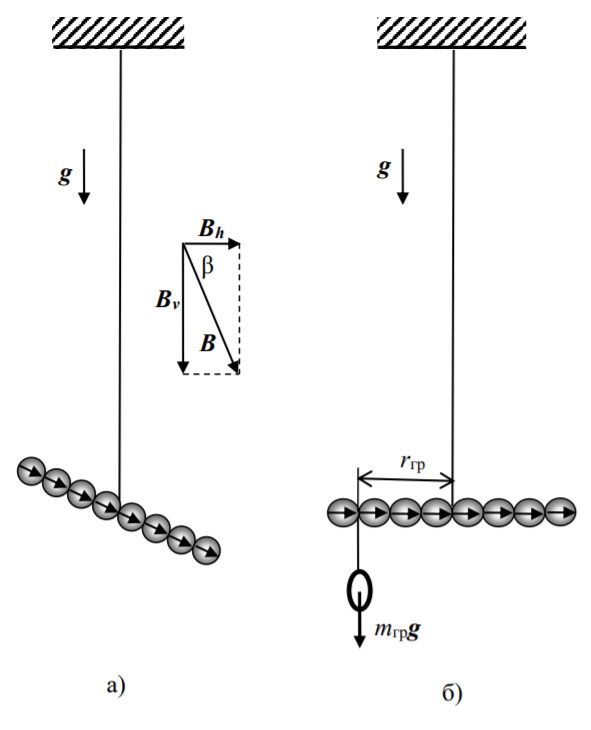
\includegraphics[scale=0.7]{Pictures/Вер.png}
\end{figure}

Для измерения вертикальной составляющей вектора индукции поля Земли используется та же установка, что и для измерения горизонтальной составляющей с тем лишь отличием, что магнитная «стрелка» подвешивается на нити без $\Lambda$-образного подвеса. В этом случае магнитная «стрелка», составленная из чётного числа шариков и подвешенная на тонкой нити за середину, расположится не горизонтально, а под некоторым, отличным от нуля, углом к горизонту.

С помощью небольшого дополнительного грузика «стрелку» можно «выровнять», расположив её горизонтально: в этом случае момент силы тяжести груза относительно точки подвеса будет равен моменту сил, действующих на «стрелку» со стороны магнитного поля Земли.
\vspace{15mm}

Выпишем все необходимые формулы.

Сила взаимодействия двух небольших постоянных магнитов, направленных вдоль прямой, соединяющей их:

\begin{equation*}
	F = -6\frac{P_m^2}{r^4}
\end{equation*}

индукция магнитного поля $\overrightarrow{B_p}$ на полюсах однородно намагниченного шара связана с величиной намагниченности $\overrightarrow{p}_m$ и остаточной магнитной индукцией $\overrightarrow{B_r}$ формулой:

\begin{equation*}
	\overrightarrow{B_p} = (8\pi /3)\overrightarrow{p_m} = \frac{2}{3}\overrightarrow{B_r}.
\end{equation*}


В магнитном поле с индукцией $\overrightarrow{B}$ на точечный магнитный диполь $\overrightarrow{P_m}$ действует механический момент сил:

\begin{equation*}
	\overrightarrow{M} = \overrightarrow{P_m} \times \overrightarrow{B}
\end{equation*}

Период колебаний крутильного маятника в зависимости от количества шаров:

\begin{equation*}
	T(n) = n \cdot \pi\sqrt{\frac{md^2}{3P_mB_h}}
\end{equation*}

Момент силы тяжести, уравновешивающего груза в зависимости от количества шаров:

\begin{equation*}
	M(n) = n \cdot P_mB_{\nu}
\end{equation*}


\newpage
\textbf{Ход работы:}

\vspace{5mm}
Берем два неодимовых шарика массой $\thicksim 820$ г каждый.

Получаем $m = (820 \pm 1)$ г.

Их диаметр $d = (5,9 \pm 0,1)$ мм.

Найдем расстояние $r_{max}$, на котором сила их взаимодействия пренебрежимо слаба.

Подкладывая листочки между шариками, экспериментально получаем $r_{max} = (23,9 \pm 0,1)$ мм.

Отсюда можно найти величину магнитного момента одного шарика:

\begin{equation*}
	P_m = \sqrt{\frac{mgr_{max}^4}{6}} \approx 6,6 \cdot 10^{-2} \text{ А}\cdot \text{м}^2
\end{equation*}
\begin{equation*}
	\sigma_{P_m} = P_m \sqrt{\frac{1}{4}\left(\frac{\sigma_m}{m}\right)^2 + 4\left(\frac{\sigma_r}{r}\right)^2} \approx 0,2 \cdot 10^{-2} \text{ А}\cdot \text{м}^2.
\end{equation*}

Итого:
\begin{equation*}
	P_m = (6,6 \pm 0,2)\cdot 10^{-2} \text{ А}\cdot \text{м}^2.
\end{equation*}
\vspace{7mm}

Измерим горизонтальную составляющую магнитного поля Земля по периоду крутильных колебаний маятника.
Для этого снимем зависимость периода колебаний $T$ от количества шариков $n$.
Получаем следующую таблицу: 


\begin{table}[h!]
	\centering
	\renewcommand{\tabcolsep}{1.5cm}
	\begin{tabular}{|c|c|c|}
		\hline
		$n$                 & $5T$, с & $\overline{T}$, с     \\ \hline
		\multirow{3}{*}{7}  & 9,86    & \multirow{3}{*}{1,95} \\ \cline{2-2}
		& 9,61    &                       \\ \cline{2-2}
		& 9,79    &                       \\ \hline
		\multirow{3}{*}{8}  & 11,23   & \multirow{3}{*}{2,27} \\ \cline{2-2}
		& 11,27   &                       \\ \cline{2-2}
		& 11,03   &                       \\ \hline
		\multirow{3}{*}{9}  & 11,83   & \multirow{3}{*}{2,40} \\ \cline{2-2}
		& 12,01   &                       \\ \cline{2-2}
		& 12,21   &                       \\ \hline
		\multirow{3}{*}{10} & 13,11   & \multirow{3}{*}{2,67} \\ \cline{2-2}
		& 13,11   &                       \\ \cline{2-2}
		& 13,76   &                       \\ \hline
		\multirow{3}{*}{11} & 14,22   & \multirow{3}{*}{2,86} \\ \cline{2-2}
		& 14,03   &                       \\ \cline{2-2}
		& 14,70   &                       \\ \hline
	\end{tabular}
\end{table}
\newpage

Строим график $T(n) = kn$. Получаем следующее:

\begin{figure}[h!]
	\centering
	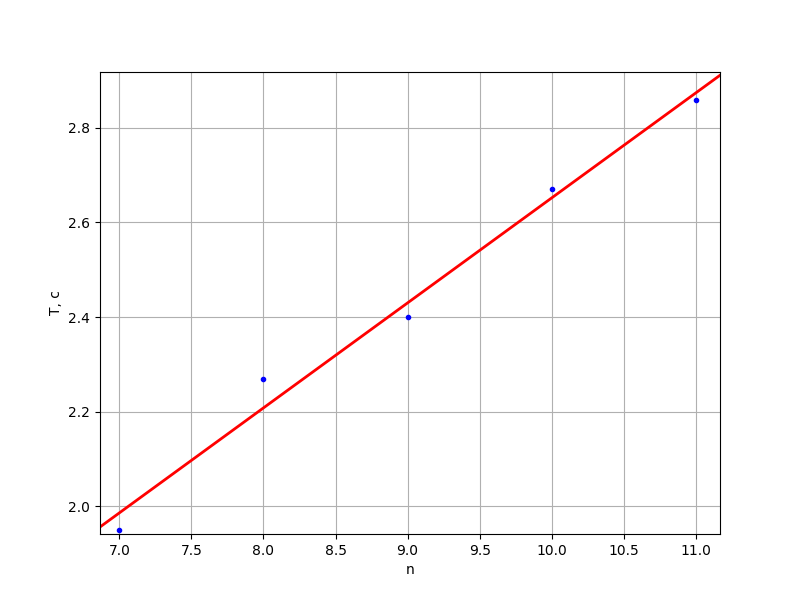
\includegraphics[scale=0.8]{Pictures/T(n).png}
\end{figure}

По МНК получаем для коэффициента наклона:

$k = (0,269 \pm 0,02)$ с.

Тогда горизонтальная составляющая магнитного поля Земли:
\begin{equation*}
	B_h = \frac{\pi ^2 md^2}{3P_m k^2} \approx 19,6 \text{ мкТл}.
\end{equation*}

\begin{equation*}
	\sigma_{B_h} = B_h \sqrt{\left(\frac{\sigma_m}{m}\right)^2 + 4\left(\frac{\sigma_d}{d}\right)^2 + \left(\frac{\sigma_{P_m}}{P_m}\right)^2 + 4 \left(\frac{\sigma_k}{k}\right)} \approx 2,9 \text{ мкТл}.
\end{equation*}

Итого:

\begin{equation*}
	B_h = (19,6 \pm 2,9) \text{ мкТл}.
\end{equation*}

\newpage

Теперь найдем вертикальную составляющую магнитного поля Земли двумя способами.

1) По углу наклона линии из 12 шариков.

\begin{figure}[h!]
	\centering
	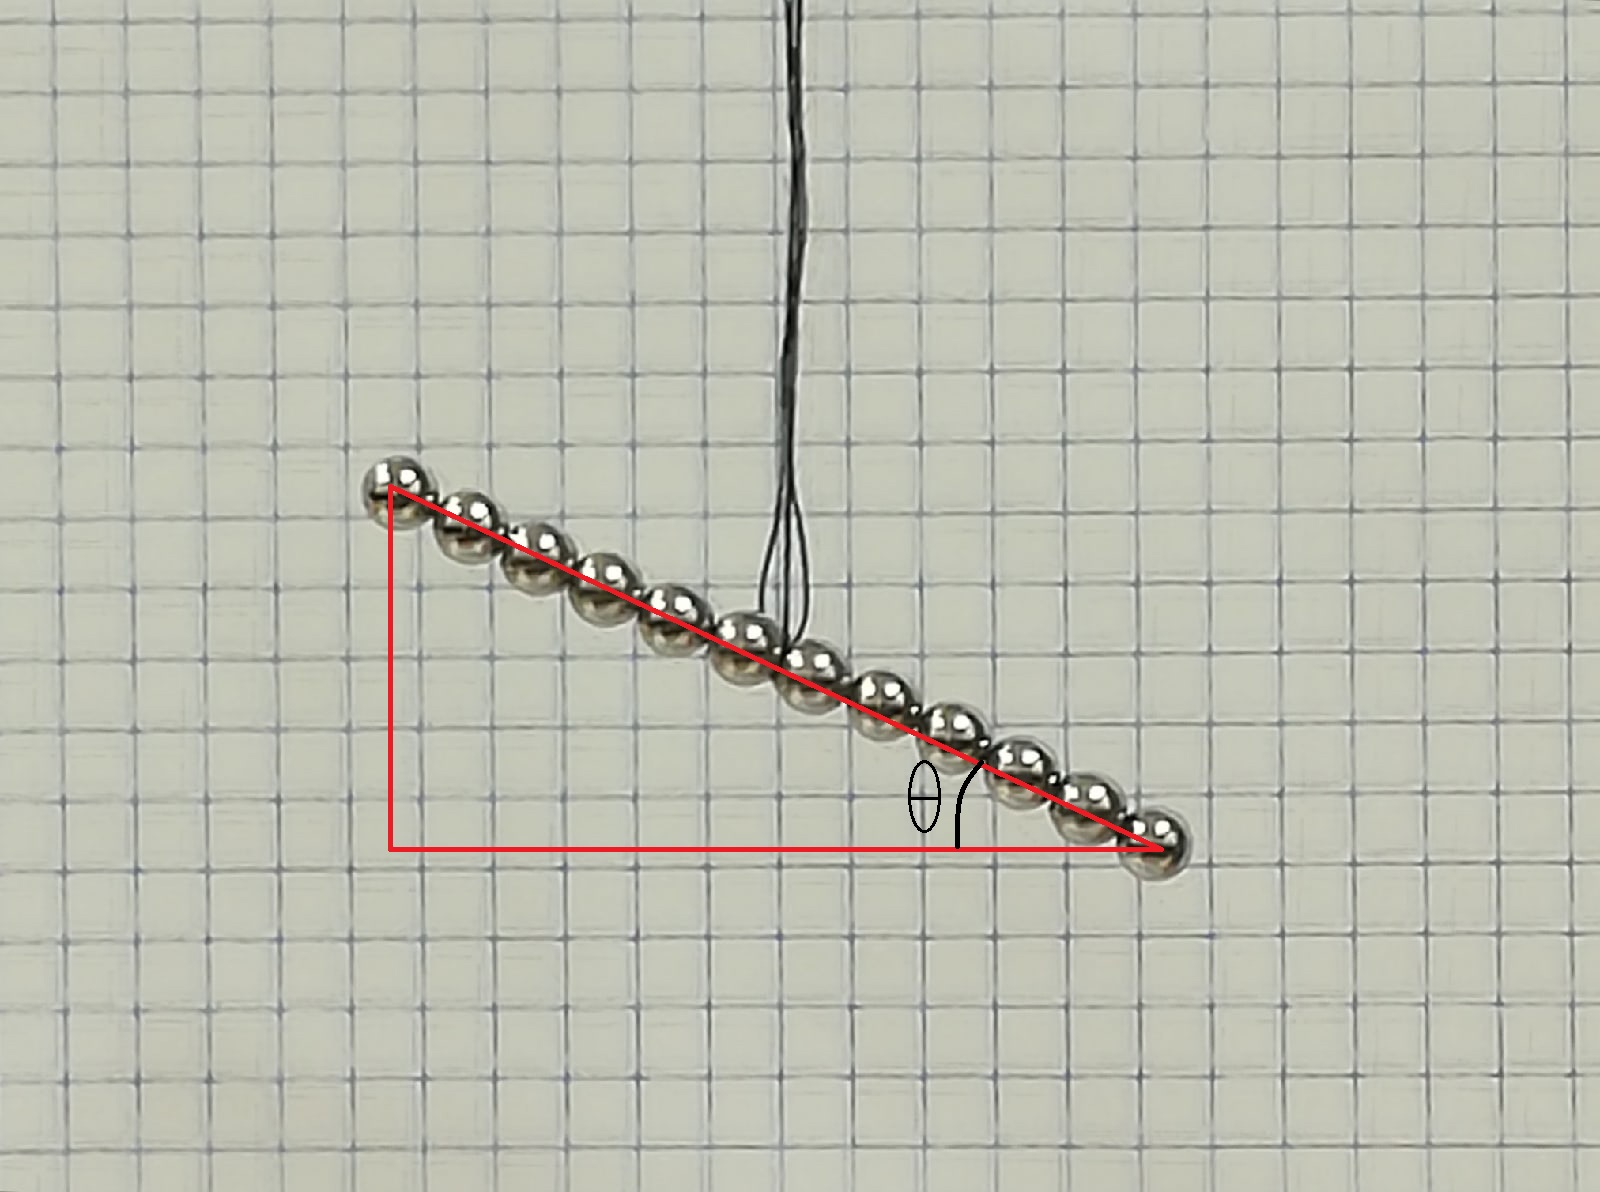
\includegraphics[scale=0.5]{Pictures/angleMes.jpg}
\end{figure}

Из рисунка видно, что $\tg\theta \approx 0,5$. Откуда $B_{\nu} = \frac{B_h}{\tg\theta} \approx 39,6$ мкТл.

\vspace{10mm}
2) Подвешивание грузика.

Подвесим грузик такой массы $m_{\text{гр}}$ на расстоянии от точки подвеса $r_{\text{гр}}$, чтобы линия из шариков была горизонтальна.

В нашем случае $m_{\text{гр}} = 128$ мг, $r_{\text{гр}} = 5d = 29,5$ мм.

Получаем: $B_{\nu} = \frac{m_{\text{гр}}gr_{\text{гр}}}{nP_m} \approx 47$ мкТл.

\vspace{12mm}

Как видим, результаты по обоим способам достаточно близки друг к другу.

Среднее $\overline{B_{\nu}} = 43,3$ мкТл.

Значит полное поле Земли $B = \sqrt{B_{h}^2 + B_{\nu}^2} \approx 47,5$ мкТл, что почти совпадает с табличным значением магнитного поля в г.Долгопрудном $B_{\text{табл}} = 50$ мкТл.

\newpage
\begin{figure}[h!]
	\centering
	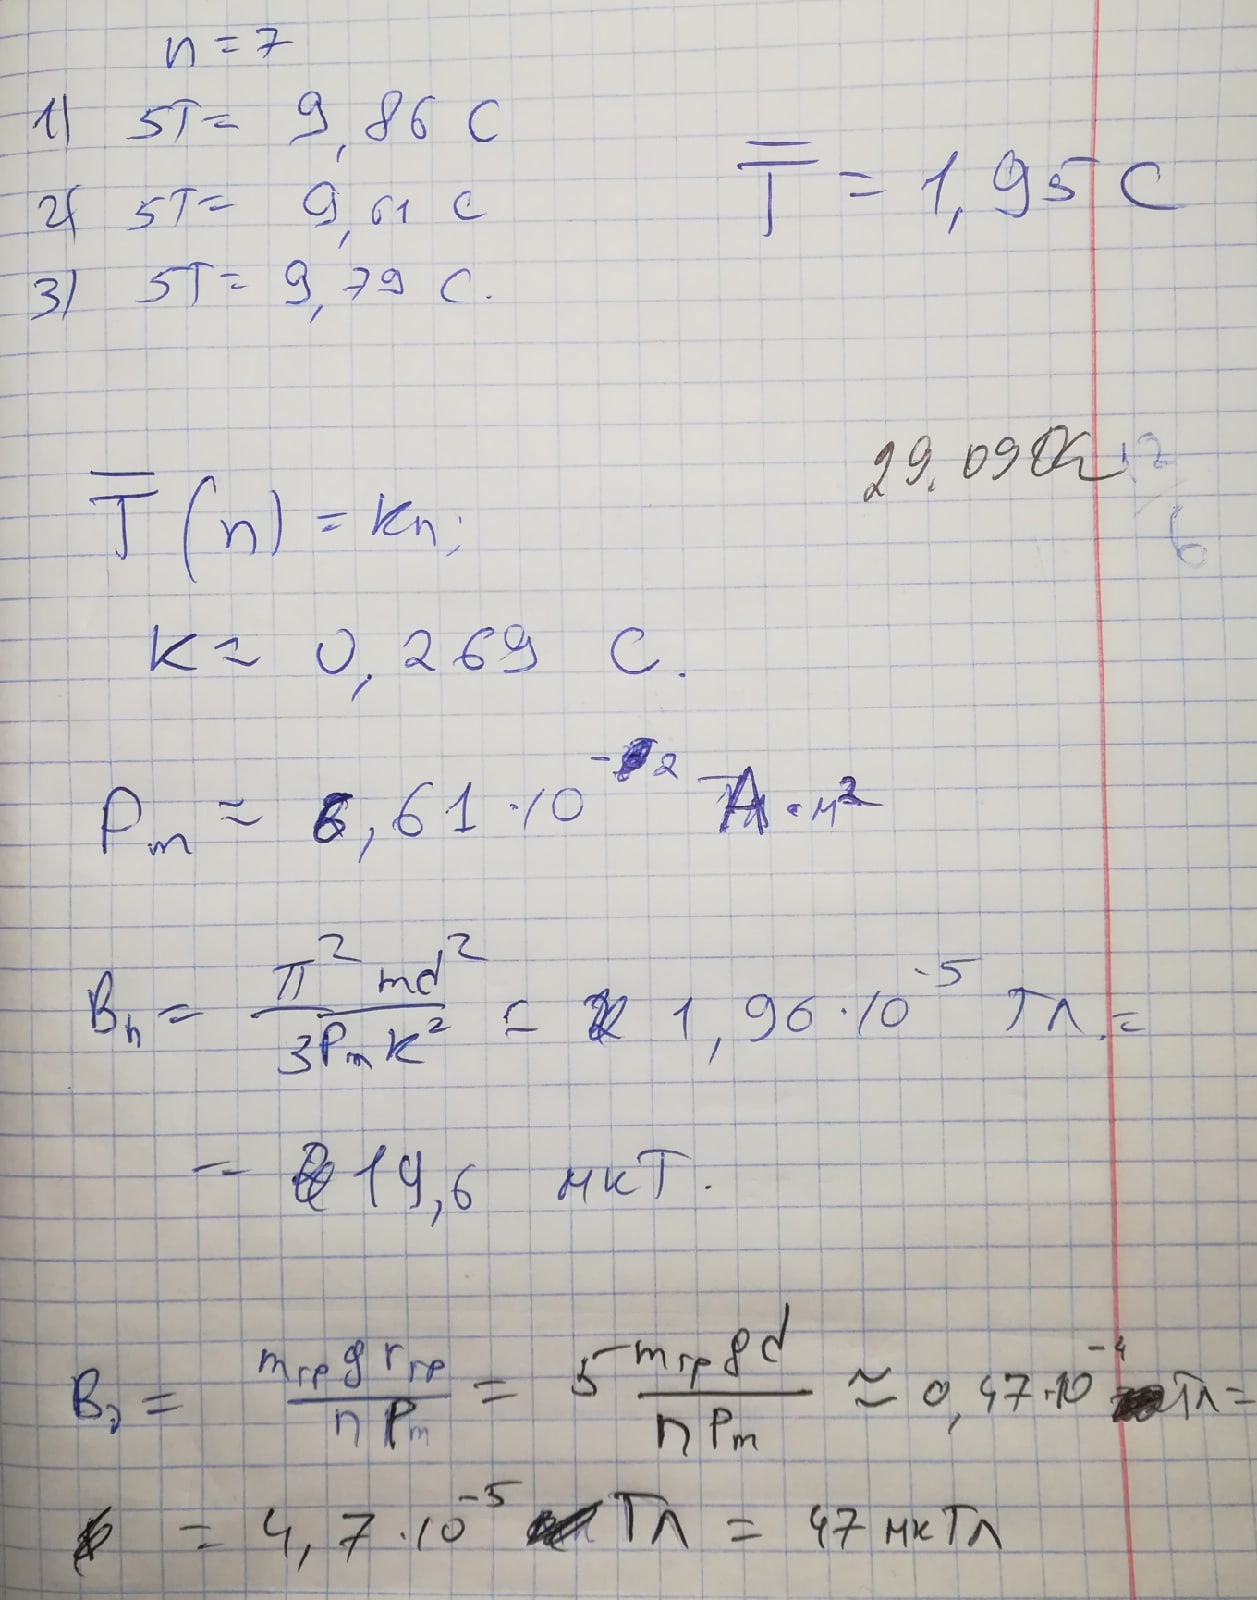
\includegraphics[scale=0.32]{Pictures/sign.jpg}
\end{figure}
Исследуем зависимость магнитного поля соленоида от количества магнитиков толщиной $h = 4$ мм и радиусом $R = 4,5$ мм.

\begin{figure}[h!]
	\centering
	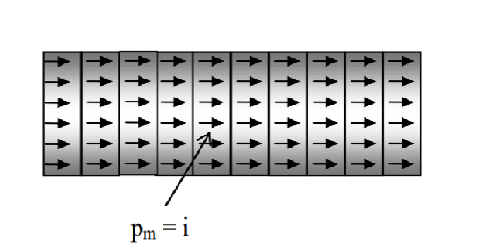
\includegraphics[scale=0.7]{Pictures/Цил.png}
\end{figure}

\begin{table}[h!]
	\centering
	\begin{tabular}{|c|c|c|}
		\hline
		$n$ & $B$, убывание & $B$, возрастание \\ \hline
		8   & 361           & 369              \\ \hline
		7   & 359           & 364              \\ \hline
		6   & 350           & 363              \\ \hline
		5   & 344           & 362              \\ \hline
		4   & 354           & 355              \\ \hline
		3   & 336           & 349              \\ \hline
		2   & 317           & 314              \\ \hline
		1   & 231           & 232              \\ \hline
	\end{tabular}
\end{table}

Построим графики. По оси абсцисс количество магнитов, а по оси ординат - индукция магнитного поля (мТл).
\begin{figure}[h!]
	\centering
	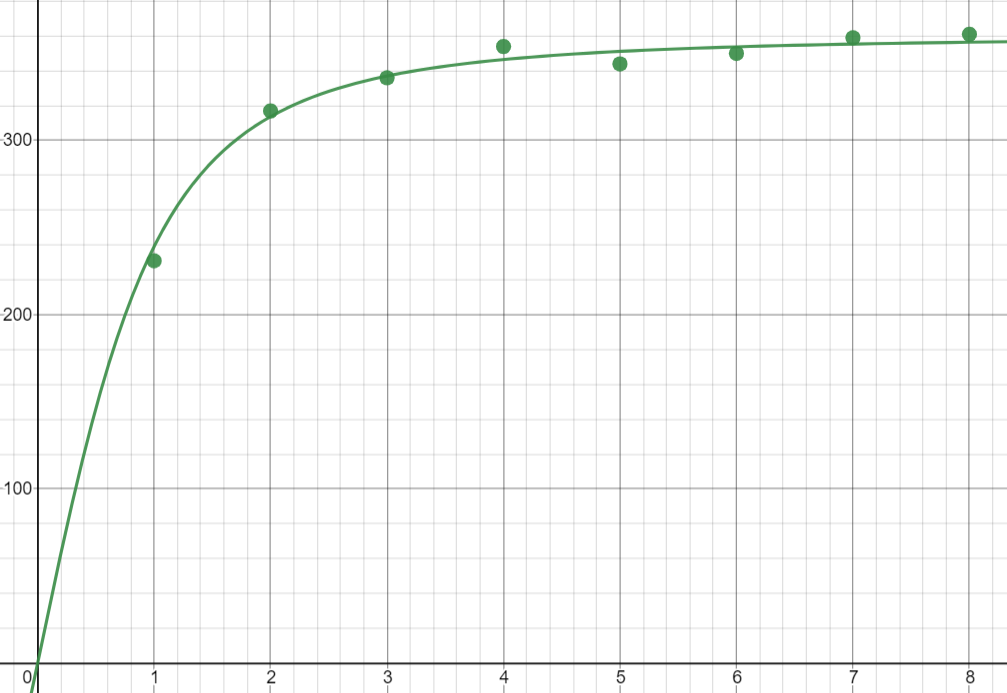
\includegraphics[scale=0.7]{Pictures/убыв.png}
	\caption*{Убывание}
\end{figure}
\vspace{15mm}

То же самое на возрастание количества магнитиков.
\begin{figure}[h!]
	\centering
	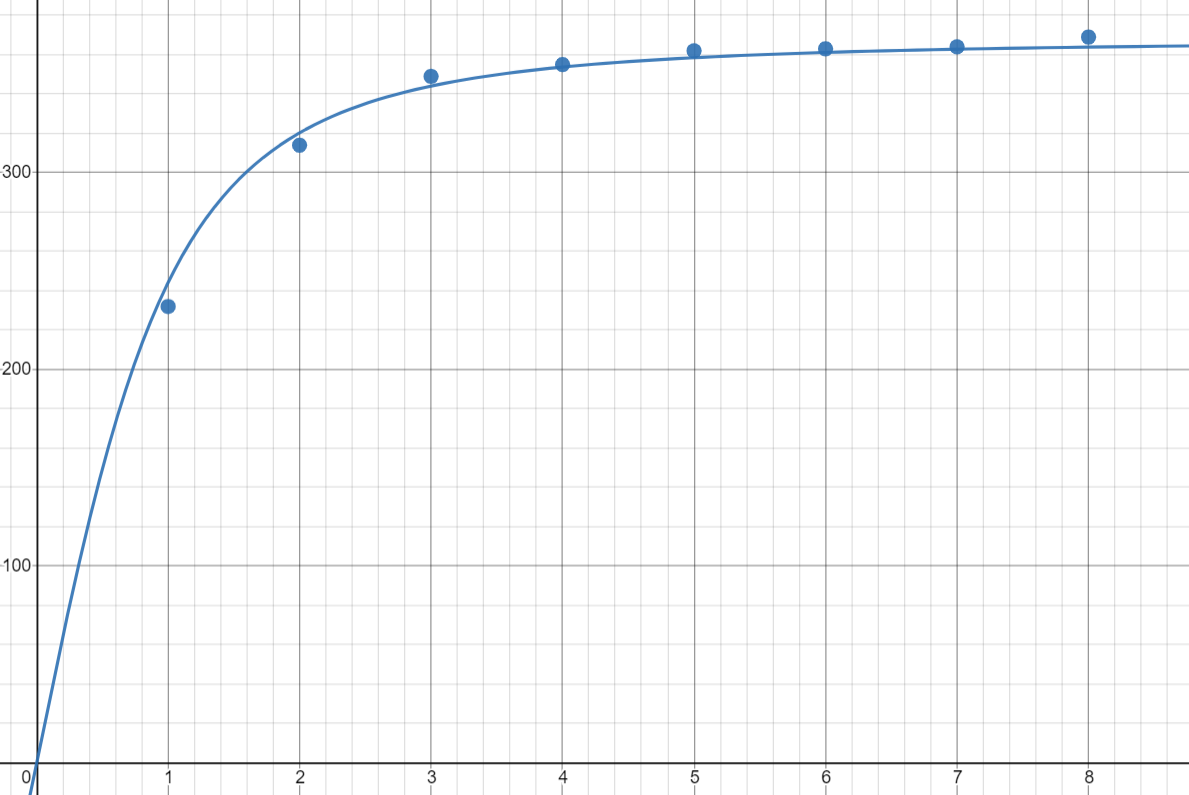
\includegraphics[scale=0.58]{Pictures/возраст.png}
	\caption*{Возрастание}
\end{figure}
\vspace{35mm}


И сразу оба:
\begin{figure}[h!]
	\centering
	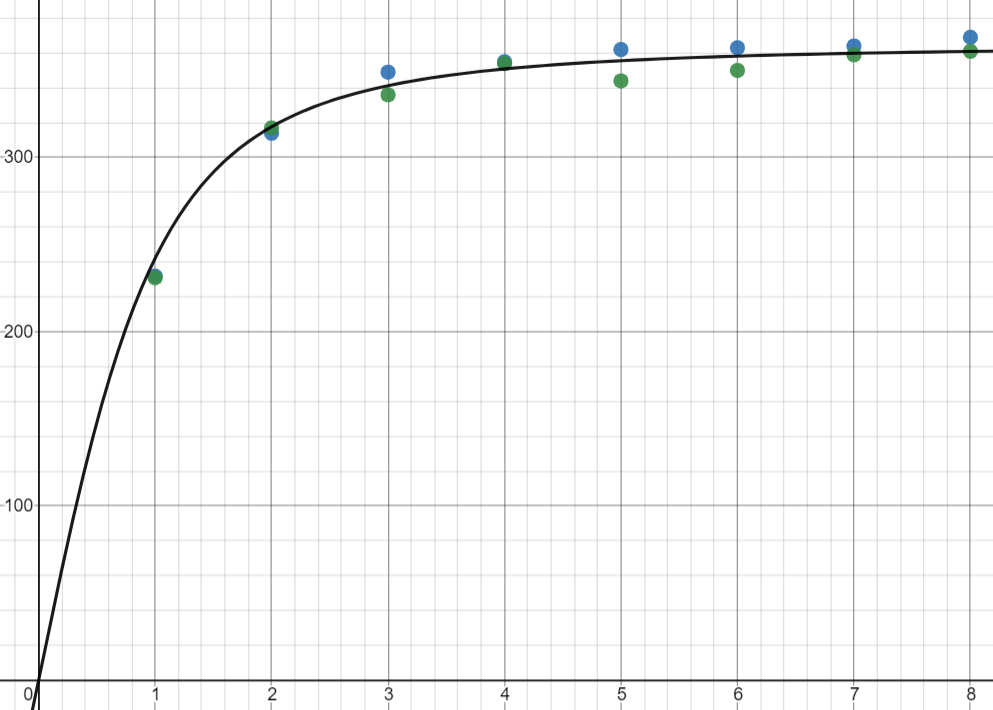
\includegraphics[scale=0.7]{Pictures/оба.png}
	\caption*{Оба}
\end{figure}
\newpage


Как видно из графиков, зависимость подчиняется закону вида 

$B(n) = C_0\cdot \frac{n}{\sqrt{C_1^2 + n^2}}$, что подтверждает теорию.

Теоретически, зависимость такая:

$B(n) = \frac{B_r}{2}\frac{nh}{\sqrt{R^2 + (nh)^2}}$.

Из обоих же графиков видно, что при $h \longrightarrow \infty$ магнитное поле соленоида $B \longrightarrow \frac{B_r}{2} \approx 370$ мТл. Откуда $B_r \approx 740$ мТл.

\vspace{30mm}

\textbf{{\normalsize Вывод:}} в данной работе были определены характеристики шарообразных неодимовых магнитов: $m = (820 \pm 1)$ г, $d = (5,9 \pm 0,1)$ мм, 

\noindent $P_m = (6,6 \pm 0,2) \cdot 10^{-2} \text{ А} \cdot \text{м}^2$. Были найдены горизонтальная и вертикальная составляющие магнитного поля Земли соответственно: $B_h = (19,6 \pm 2,9)$ мкТл, $B_{\nu} = 43,3$ мкТл; а также полное магнитное поле Земли $B = 47,5$ мкТл, что неплохо соответствует табличному значению $B_{\text{табл}} = 50$ мкТл для г.Долгопрудного. Помимо этого, в данной работе была исследована зависимость магнитного поля соленоида - в нашем случае цилиндрика из соединенных магнитов - от количества этих самых магнитов, то есть от длины соленоида, и получено предельное значение поля такого соленоида $B_r \approx 740$ мТл. Все ошибки связаны с неточностью измерения.

\end{document}